\documentclass{beamer}
\usepackage[utf8]{inputenc}
\usepackage{hyperref}
\usepackage{multirow}

\title{Computação em Nuvem - Aula 9}
\subtitle{Provedores de computação em nuvem \\
Prof. Me. Juliana Costa-Silva}

\usetheme{lucid}

\begin{document}
\frame{
 \titlepage
}

\frame{
    \frametitle{Roteiro de Aula}
    \tableofcontents
}

%-------------------------------------------
\section{Introdução}
\begin{frame}{Como escolher o provedor?}
    
   $ \Rightarrow$ Você conhece os modelos utilizados pelos provedores para determinar os preços dos serviços? \\
   \vspace{0.5cm}
   $\Rightarrow$ Uma das características da computação em nuvem é o pagamento baseado no uso. Mas quais são as métricas utilizadas para contabilizar uso dos recursos de TI?
    
\end{frame}
%----------------------------------------
\begin{frame}{Serviços IaaS}

\begin{center}
	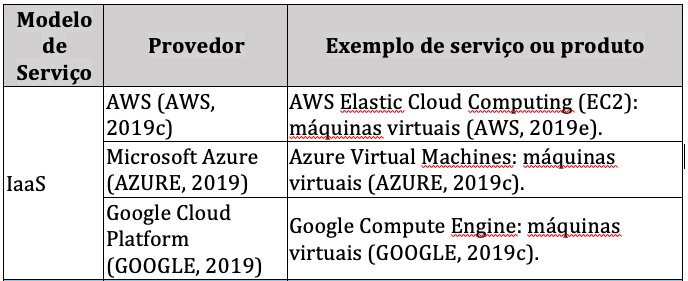
\includegraphics[height=0.47\paperheight]{fig/aula9/IaaS.png} \\
	Fonte: \cite{malheiros2019cc}
      \end{center}
    
\end{frame}
%----------------------------------------
\begin{frame}{Serviços PaaS}

\begin{center}
	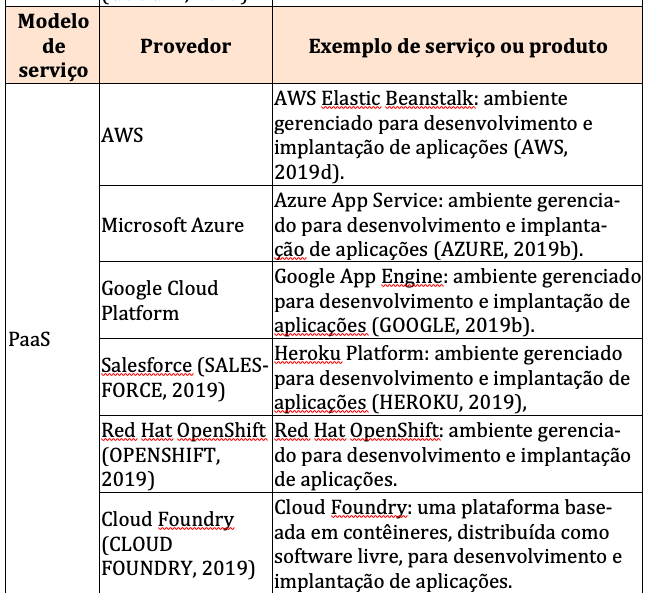
\includegraphics[width=0.75\paperheight]{fig/aula9/PaaS.png} \\
	Fonte: \cite{malheiros2019cc}
      \end{center}
    
\end{frame}
%----------------------------------------
\begin{frame}{Serviços SaaS}

\begin{center}
	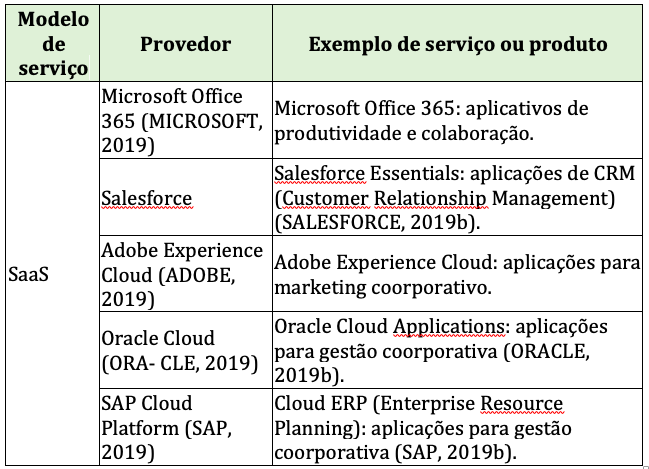
\includegraphics[height=0.6\paperheight]{fig/aula9/SaaS.png} \\
	Fonte: \cite{malheiros2019cc}
      \end{center}
    
\end{frame}
%-------------------------------------------
\section{Atividade PARCIAL}
\begin{frame}{Atividade - PARCIAL}
    
    $\Rightarrow$ Pesquise cada sistema indicado e indique como são tarifados;\\
    \vspace{0.5cm}
    $\Rightarrow$ Indique os pontos que geram dúvida na cobrança;\\
    \vspace{0.9cm}
     \textbf{DESENVOLVA a Atividade no AVA, \textcolor{red}{Unidade 3 - Seção 2}\\
Esta atividade é nota PARCIAL;}
    
\end{frame}
%----------------------------------------
%----------------------------------------
\begin{frame}{Referências}%[allowframebreaks]
 \tiny
 \begin{center}
 	\bibliographystyle{apalike}
	 \bibliography{ref}
 \end{center}
 \end{frame}

\end{document}